\chapter{Anhang}
\label{ch:anhang}

\begin{figure}[h]
	\vspace{2cm}
	\begin{subfigure}{\textwidth}
		\centering
		\begin{tabular}{|c|c|}
			\hline Bauteil & Wert \\ 
			\hline R1 & $50 \ k\Omega$ \\ 
			\hline R2 & $50 \ k\Omega$ \\ 
			\hline C1 & $380 \ pF$ \\ 
			\hline C2 & $10 \ nF$ \\ 
			\hline 
		\end{tabular} 
		\caption{Wertetabelle für die Timerbauteile in Schaltung \ref{fig:schaltplan_ne555} laut Berechnungsformel aus Quelle \cite{ELKO}}
		\label{fig:wertetabelle_ne555}
	\end{subfigure}
	\par\bigskip
	\vspace{1.5cm}
	\centering
	\begin{subfigure}{\textwidth}[h]
		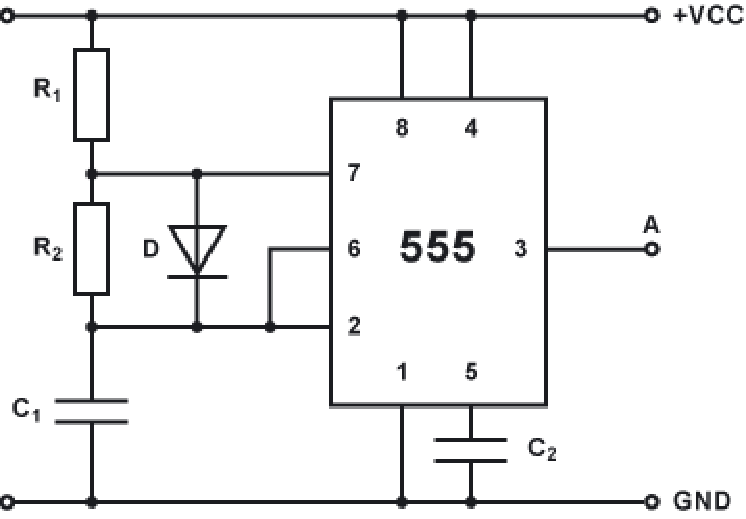
\includegraphics[height=.4\textheight]{images/ne555_astabile_kippstufe.pdf}
		\caption{Schaltplan des Timerbausteins \cite{ELKO}}
		\label{fig:schaltplan_ne555}
	\end{subfigure}
\end{figure}
\begin{figure}[h]
	\ContinuedFloat
	\centering
	\begin{subfigure}{\textwidth}
		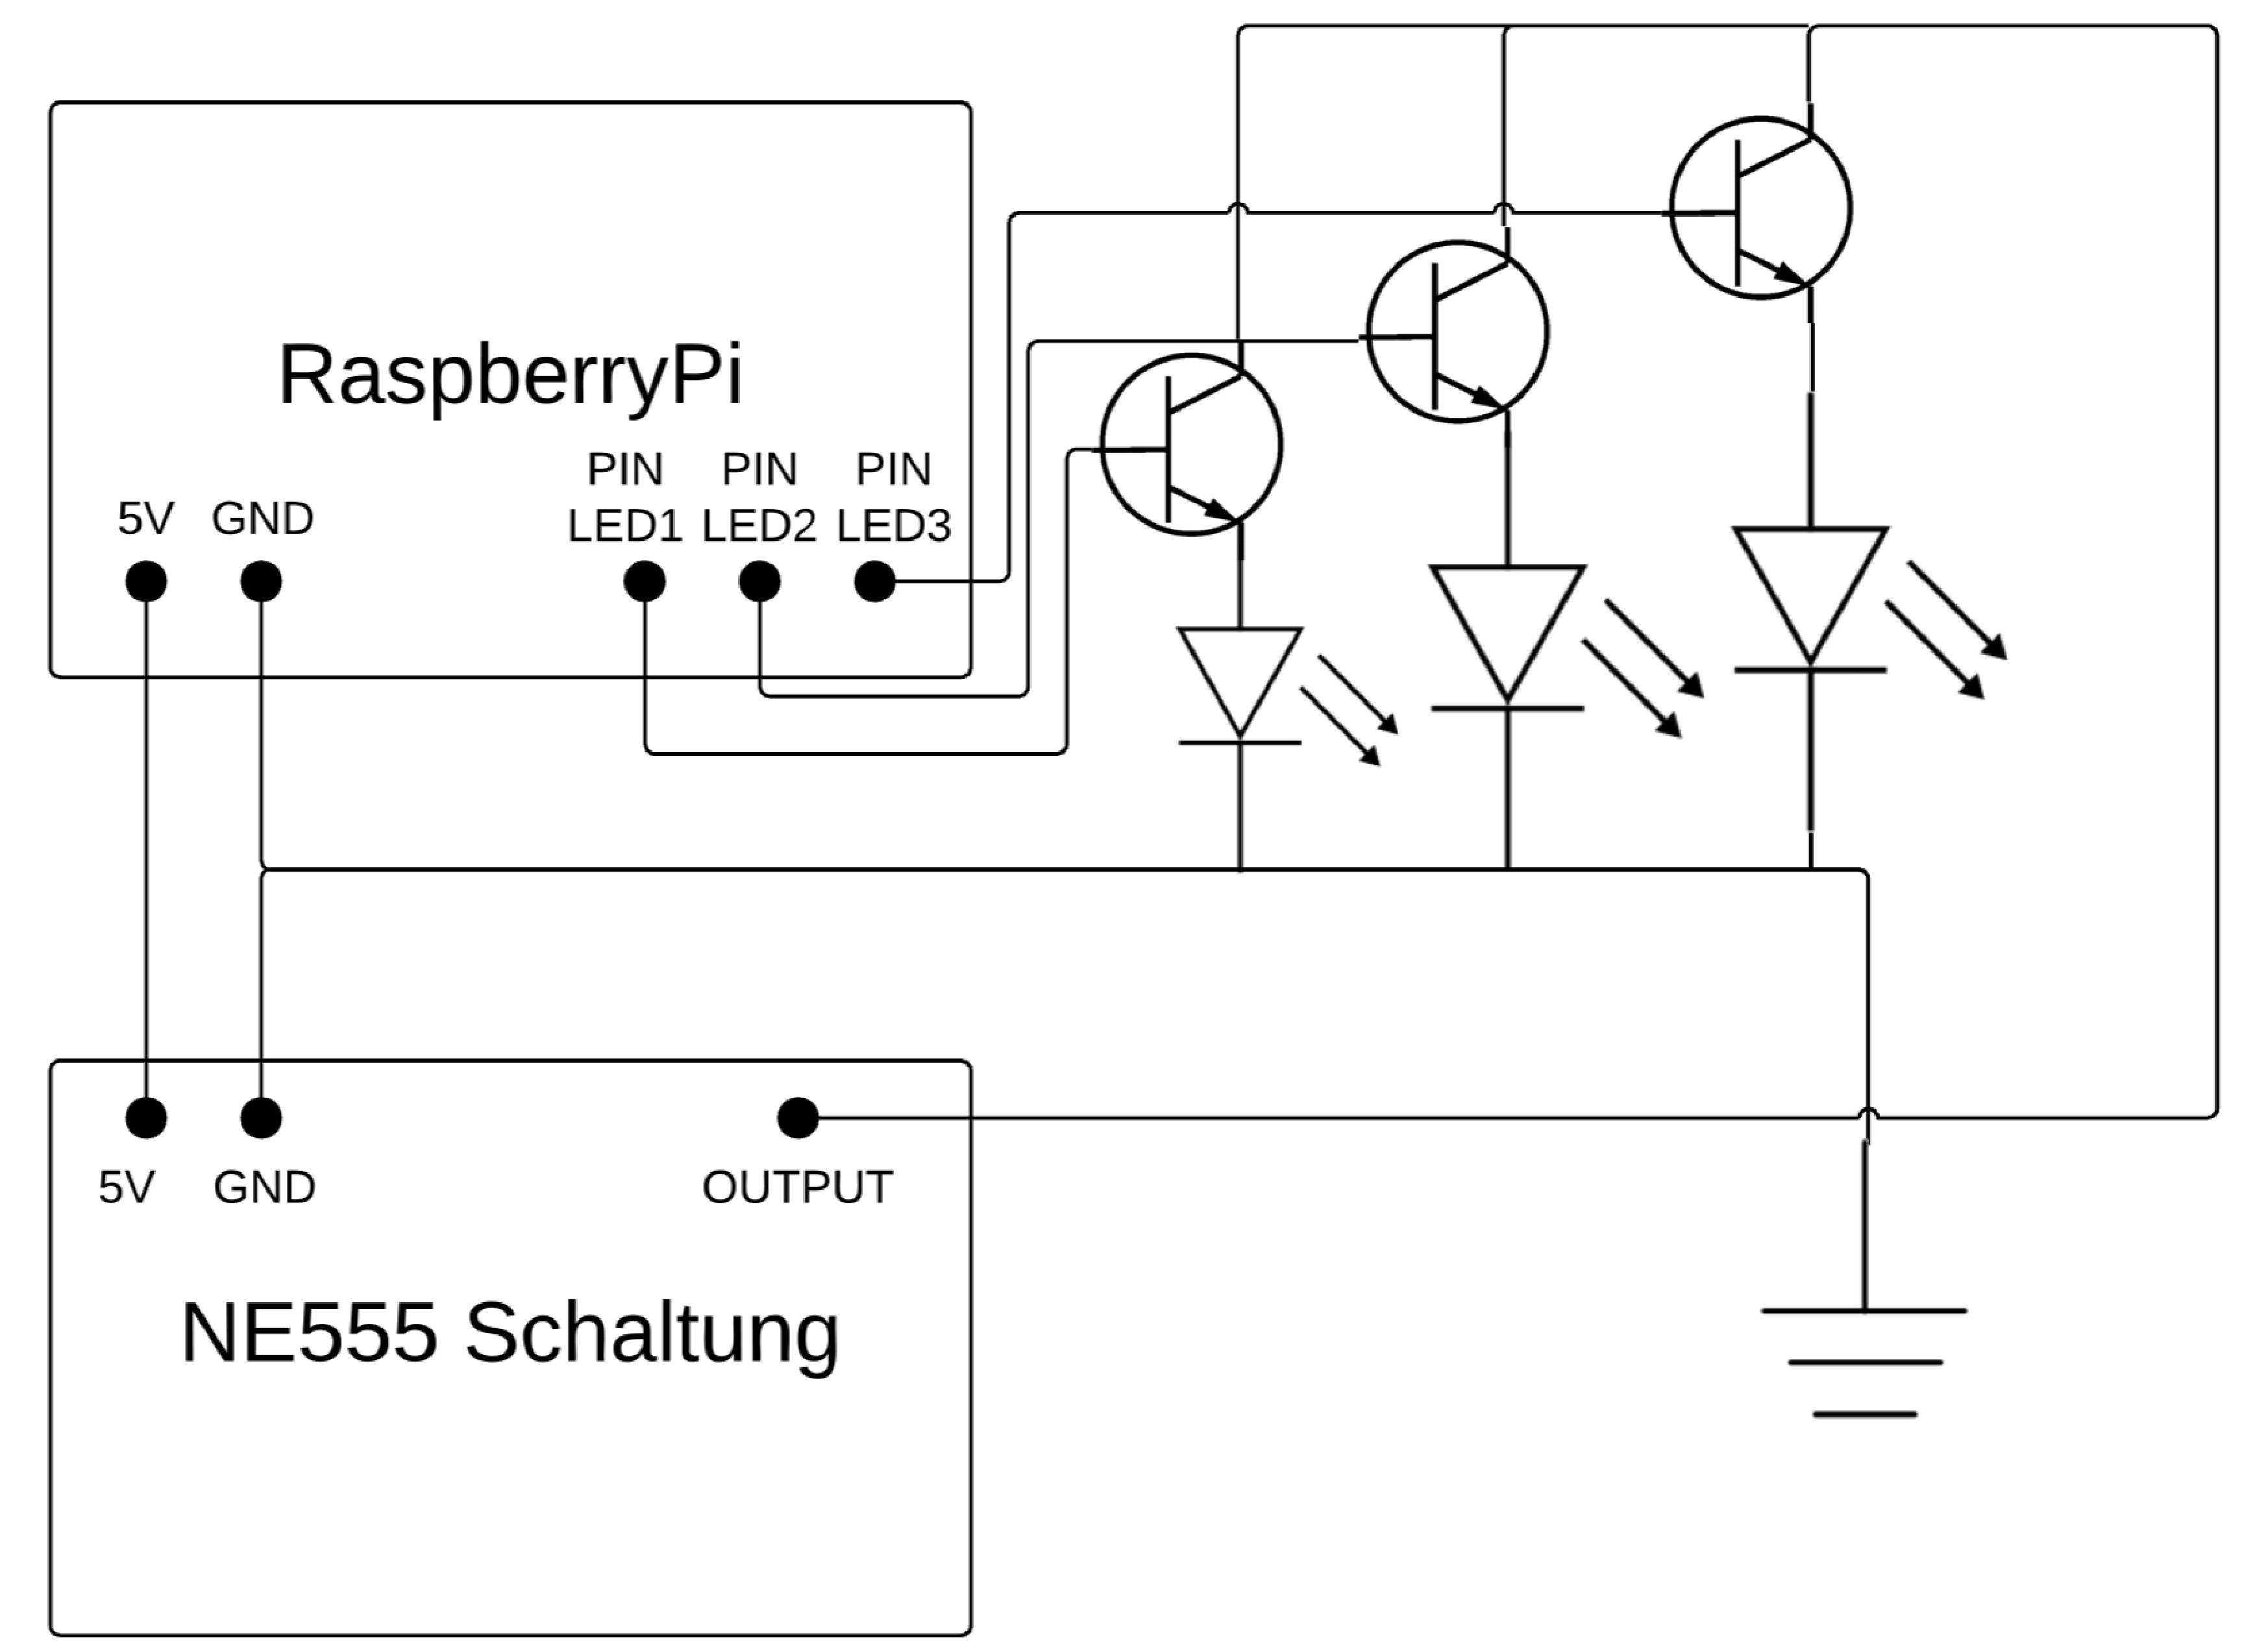
\includegraphics[height=.4\textheight]{images/schaltung_ne555_led.pdf}
		\caption{Gesamter Schaltplan der Infrarot-LEDs}
		\label{fig:schaltplan_ne555_leds}
	\end{subfigure}
\end{figure}



\begin{figure}
	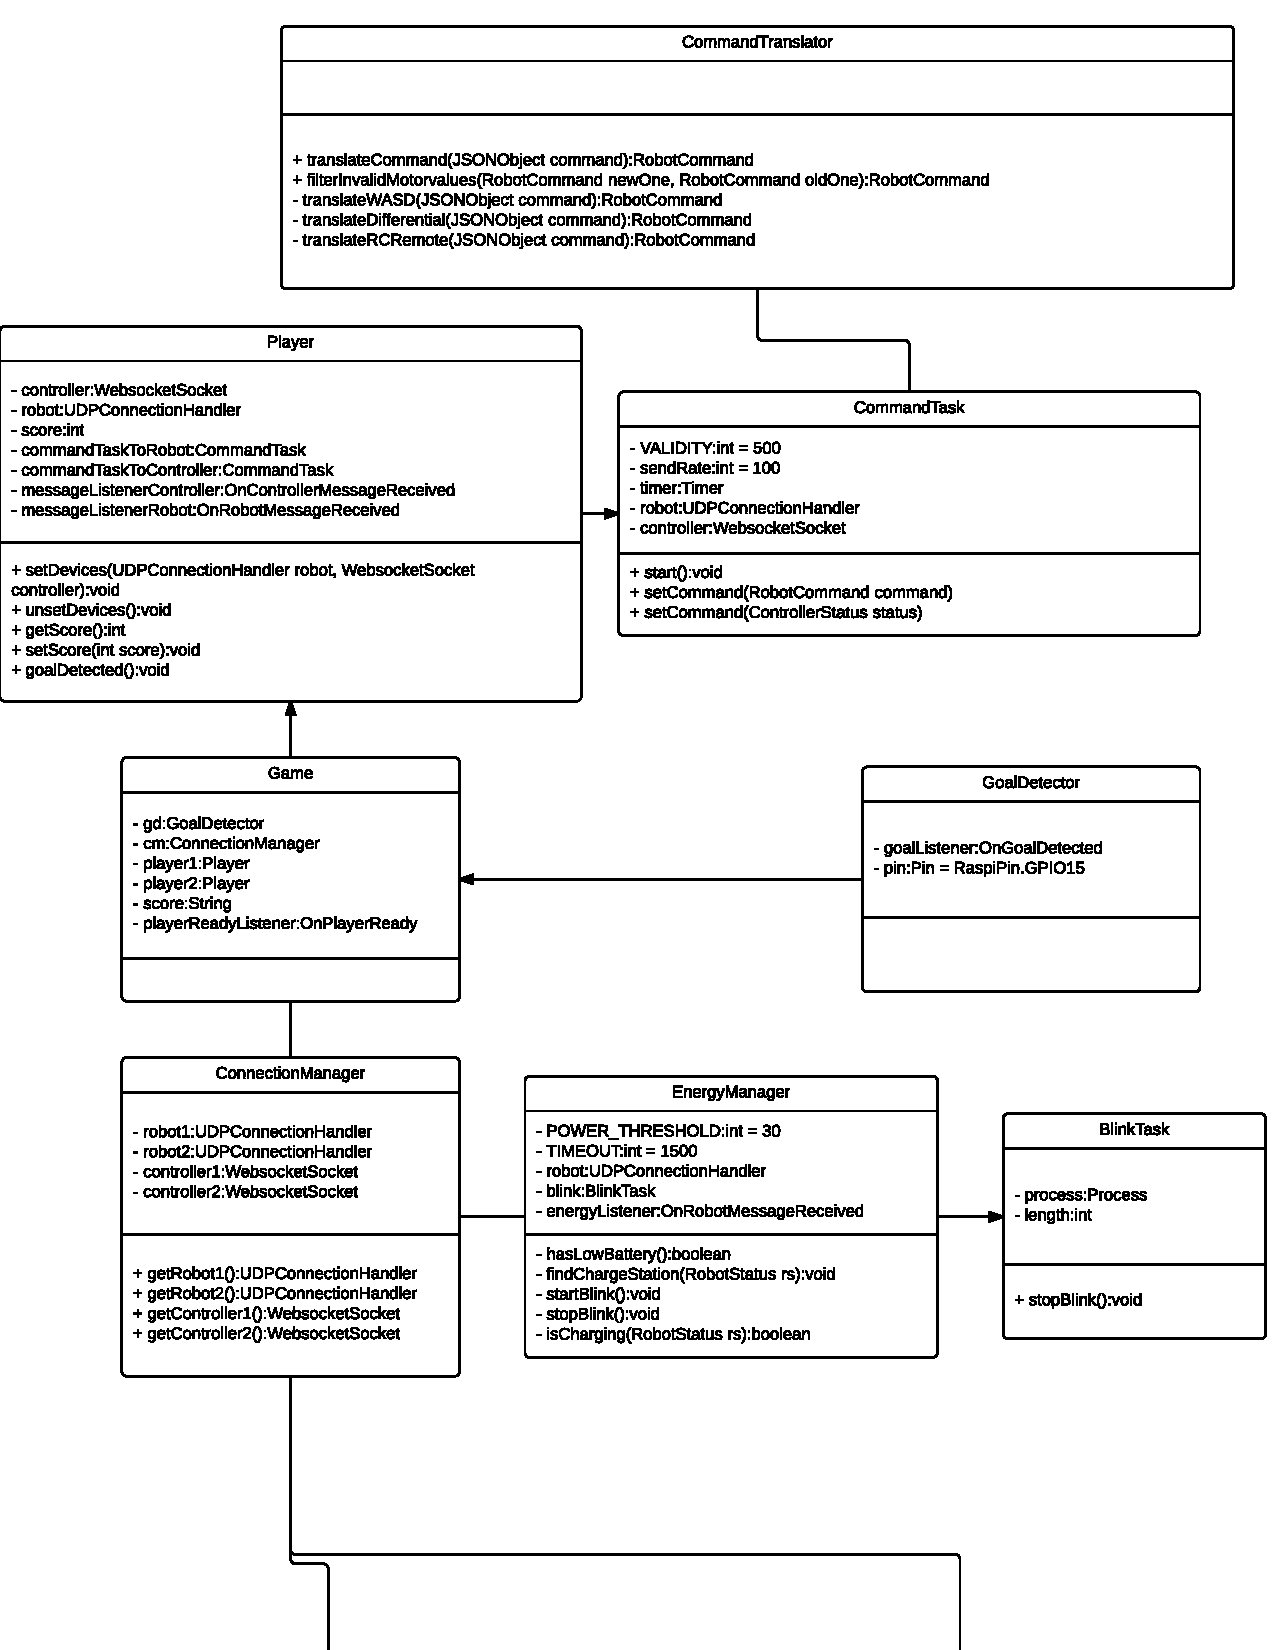
\includegraphics[page=1,width=\textwidth]{images/uml_software_all.pdf}

\end{figure}
\begin{figure}
	\includegraphics[page=2,width=\textwidth]{images/uml_software_all.pdf}
	
	\caption{Klassendiagramm des Servers}
	\label{fig:server_uml_all}
\end{figure}


\begin{figure}
	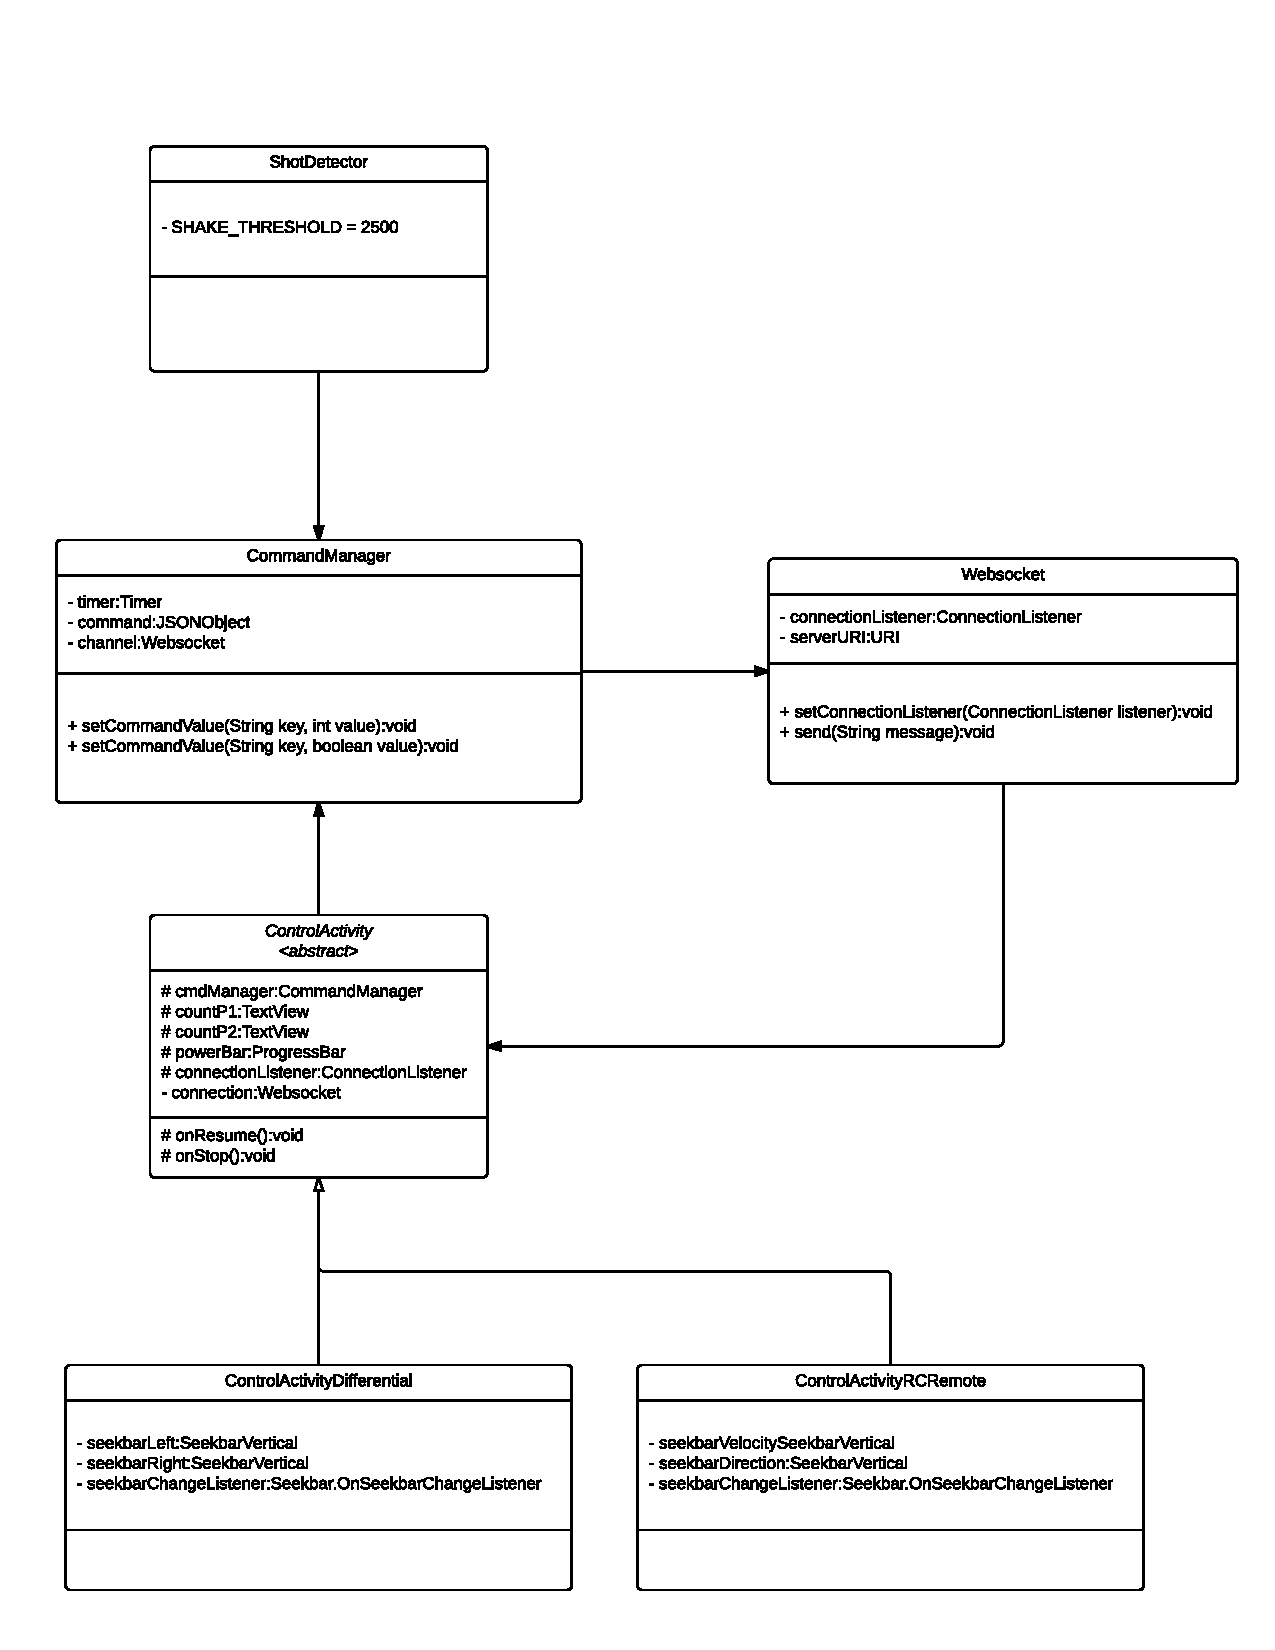
\includegraphics[width=\textwidth]{images/uml_android_app.pdf}
	\caption{Klassendiagramm der Android Anwendung}
	\label{fig:android_uml}
\end{figure}

